\usetikzlibrary{decorations.pathmorphing,decorations.markings}
\providecommand{\ket}[1]{\left|#1\right\rangle}
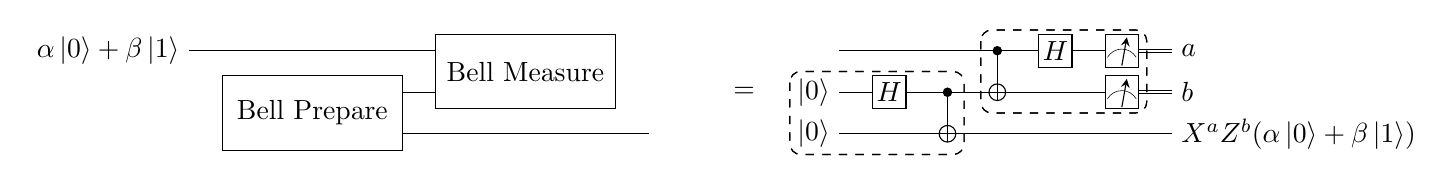
\begin{tikzpicture}[scale=1.000000,x=1pt,y=1pt]
\filldraw[color=white] (0.000000, -7.500000) rectangle (397.000000, 37.500000);
% Drawing wires
% Line 11: x W \alpha\ket{0}+\beta\ket{1} {} {} {a}
\draw[color=black] (13.500000,30.000000) -- (142.500000,30.000000);
\draw[color=white] (142.500000,30.000000) -- (194.500000,30.000000);
\draw[color=black] (248.500000,30.000000) -- (358.000000,30.000000);
\draw[color=black] (358.000000,29.500000) -- (383.500000,29.500000);
\draw[color=black] (358.000000,30.500000) -- (383.500000,30.500000);
% Line 12: y W \ket{0} {} {\ket{0}} {b}
\draw[color=white] (13.500000,15.000000) -- (65.500000,15.000000);
\draw[color=black] (65.500000,15.000000) -- (142.500000,15.000000);
\draw[color=white] (142.500000,15.000000) -- (194.500000,15.000000);
\draw[color=black] (248.500000,15.000000) -- (358.000000,15.000000);
\draw[color=black] (358.000000,14.500000) -- (383.500000,14.500000);
\draw[color=black] (358.000000,15.500000) -- (383.500000,15.500000);
% Line 13: z W \ket{0} {} {\ket{0}} X^{a}Z^{b}(\alpha\ket{0}+\beta\ket{1})
\draw[color=white] (13.500000,0.000000) -- (65.500000,0.000000);
\draw[color=black] (65.500000,0.000000) -- (194.500000,0.000000);
\draw[color=black] (248.500000,0.000000) -- (383.500000,0.000000);
% Done with wires; drawing gates
% Line 15: x START
\draw[color=black] (21.000000,30.000000) node[fill=white,left,minimum height=15.000000pt,minimum width=15.000000pt,inner sep=0pt] {\phantom{$\alpha\ket{0}+\beta\ket{1}$}};
\draw[color=black] (21.000000,30.000000) node[left] {$\alpha\ket{0}+\beta\ket{1}$};
% Line 16: y START y:color=white
\draw[color=white] (21.000000,15.000000) node[fill=white,left,minimum height=15.000000pt,minimum width=15.000000pt,inner sep=0pt] {\phantom{$\ket{0}$}};
\draw[color=white] (21.000000,15.000000) node[left] {$\ket{0}$};
% Line 17: z START z:color=white
\draw[color=white] (21.000000,0.000000) node[fill=white,left,minimum height=15.000000pt,minimum width=15.000000pt,inner sep=0pt] {\phantom{$\ket{0}$}};
\draw[color=white] (21.000000,0.000000) node[left] {$\ket{0}$};
% Line 19: y z G {Bell Prepare} width=65 z:color=black y:color=black
\draw (65.500000,15.000000) -- (65.500000,0.000000);
\begin{scope}
\draw[fill=white] (65.500000, 7.500000) +(-45.000000:45.961941pt and 19.091883pt) -- +(45.000000:45.961941pt and 19.091883pt) -- +(135.000000:45.961941pt and 19.091883pt) -- +(225.000000:45.961941pt and 19.091883pt) -- cycle;
\clip (65.500000, 7.500000) +(-45.000000:45.961941pt and 19.091883pt) -- +(45.000000:45.961941pt and 19.091883pt) -- +(135.000000:45.961941pt and 19.091883pt) -- +(225.000000:45.961941pt and 19.091883pt) -- cycle;
\draw (65.500000, 7.500000) node {{Bell Prepare}};
\end{scope}
% Line 20: x y G {Bell Measure} width=65 x:color=white y:color=white
\draw (142.500000,30.000000) -- (142.500000,15.000000);
\begin{scope}
\draw[fill=white] (142.500000, 22.500000) +(-45.000000:45.961941pt and 19.091883pt) -- +(45.000000:45.961941pt and 19.091883pt) -- +(135.000000:45.961941pt and 19.091883pt) -- +(225.000000:45.961941pt and 19.091883pt) -- cycle;
\clip (142.500000, 22.500000) +(-45.000000:45.961941pt and 19.091883pt) -- +(45.000000:45.961941pt and 19.091883pt) -- +(135.000000:45.961941pt and 19.091883pt) -- +(225.000000:45.961941pt and 19.091883pt) -- cycle;
\draw (142.500000, 22.500000) node {{Bell Measure}};
\end{scope}
% Line 24: x y z END
\draw[color=white] (187.000000,30.000000) node[fill=white,right,minimum height=15.000000pt,minimum width=15.000000pt,inner sep=0pt] {\phantom{${}$}};
\draw[color=white] (187.000000,30.000000) node[right] {${}$};
\draw[color=white] (187.000000,15.000000) node[fill=white,right,minimum height=15.000000pt,minimum width=15.000000pt,inner sep=0pt] {\phantom{${}$}};
\draw[color=white] (187.000000,15.000000) node[right] {${}$};
\draw[color=black] (187.000000,0.000000) node[fill=white,right,minimum height=15.000000pt,minimum width=15.000000pt,inner sep=0pt] {\phantom{${}$}};
\draw[color=black] (187.000000,0.000000) node[right] {${}$};
% Line 26: =
\draw[fill=white,color=white] (214.000000, -6.000000) rectangle (229.000000, 36.000000);
\draw (221.500000, 15.000000) node {$=$};
% Line 28: x START x:color=black
\draw[color=black] (256.000000,30.000000) node[fill=white,left,minimum height=15.000000pt,minimum width=15.000000pt,inner sep=0pt] {\phantom{${}$}};
\draw[color=black] (256.000000,30.000000) node[left] {${}$};
% Line 29: y START y:color=black
\draw[color=black] (256.000000,15.000000) node[fill=white,left,minimum height=15.000000pt,minimum width=15.000000pt,inner sep=0pt] {\phantom{${\ket{0}}$}};
\draw[color=black] (256.000000,15.000000) node[left] {${\ket{0}}$};
% Line 30: z START z:color=black
\draw[color=black] (256.000000,0.000000) node[fill=white,left,minimum height=15.000000pt,minimum width=15.000000pt,inner sep=0pt] {\phantom{${\ket{0}}$}};
\draw[color=black] (256.000000,0.000000) node[left] {${\ket{0}}$};
% Line 32: y G $H$
\begin{scope}
\draw[fill=white] (274.000000, 15.000000) +(-45.000000:8.485281pt and 8.485281pt) -- +(45.000000:8.485281pt and 8.485281pt) -- +(135.000000:8.485281pt and 8.485281pt) -- +(225.000000:8.485281pt and 8.485281pt) -- cycle;
\clip (274.000000, 15.000000) +(-45.000000:8.485281pt and 8.485281pt) -- +(45.000000:8.485281pt and 8.485281pt) -- +(135.000000:8.485281pt and 8.485281pt) -- +(225.000000:8.485281pt and 8.485281pt) -- cycle;
\draw (274.000000, 15.000000) node {$H$};
\end{scope}
% Line 33: y +z
\draw (295.000000,15.000000) -- (295.000000,0.000000);
\filldraw (295.000000, 15.000000) circle(1.500000pt);
\begin{scope}
\draw[fill=white] (295.000000, 0.000000) circle(3.000000pt);
\clip (295.000000, 0.000000) circle(3.000000pt);
\draw (292.000000, 0.000000) -- (298.000000, 0.000000);
\draw (295.000000, -3.000000) -- (295.000000, 3.000000);
\end{scope}
% Line 35: +y x
\draw (313.000000,30.000000) -- (313.000000,15.000000);
\begin{scope}
\draw[fill=white] (313.000000, 15.000000) circle(3.000000pt);
\clip (313.000000, 15.000000) circle(3.000000pt);
\draw (310.000000, 15.000000) -- (316.000000, 15.000000);
\draw (313.000000, 12.000000) -- (313.000000, 18.000000);
\end{scope}
\filldraw (313.000000, 30.000000) circle(1.500000pt);
% Line 36: x H
\begin{scope}
\draw[fill=white] (334.000000, 30.000000) +(-45.000000:8.485281pt and 8.485281pt) -- +(45.000000:8.485281pt and 8.485281pt) -- +(135.000000:8.485281pt and 8.485281pt) -- +(225.000000:8.485281pt and 8.485281pt) -- cycle;
\clip (334.000000, 30.000000) +(-45.000000:8.485281pt and 8.485281pt) -- +(45.000000:8.485281pt and 8.485281pt) -- +(135.000000:8.485281pt and 8.485281pt) -- +(225.000000:8.485281pt and 8.485281pt) -- cycle;
\draw (334.000000, 30.000000) node {$H$};
\end{scope}
% Line 37: x M; y M
\draw[fill=white] (352.000000, 24.000000) rectangle (364.000000, 36.000000);
\draw[very thin] (358.000000, 30.600000) arc (90:150:6.000000pt);
\draw[very thin] (358.000000, 30.600000) arc (90:30:6.000000pt);
\draw[->,>=stealth] (358.000000, 24.600000) -- +(80:10.392305pt);
% Line 37: x M; y M
\draw[fill=white] (352.000000, 9.000000) rectangle (364.000000, 21.000000);
\draw[very thin] (358.000000, 15.600000) arc (90:150:6.000000pt);
\draw[very thin] (358.000000, 15.600000) arc (90:30:6.000000pt);
\draw[->,>=stealth] (358.000000, 9.600000) -- +(80:10.392305pt);
% Line 42: x END
\draw[color=black] (376.000000,30.000000) node[fill=white,right,minimum height=15.000000pt,minimum width=15.000000pt,inner sep=0pt] {\phantom{${a}$}};
\draw[color=black] (376.000000,30.000000) node[right] {${a}$};
% Line 43: y END
\draw[color=black] (376.000000,15.000000) node[fill=white,right,minimum height=15.000000pt,minimum width=15.000000pt,inner sep=0pt] {\phantom{${b}$}};
\draw[color=black] (376.000000,15.000000) node[right] {${b}$};
% Line 44: z END
\draw[color=black] (376.000000,0.000000) node[fill=white,right,minimum height=15.000000pt,minimum width=15.000000pt,inner sep=0pt] {\phantom{$X^{a}Z^{b}(\alpha\ket{0}+\beta\ket{1})$}};
\draw[color=black] (376.000000,0.000000) node[right] {$X^{a}Z^{b}(\alpha\ket{0}+\beta\ket{1})$};
% Done with gates; drawing ending labels
% Done with ending labels; drawing cut lines and comments
% Line 47: y z @ 5 7 color=black style=dashed,rounded_corners=4pt
\draw[draw opacity=1.000000,fill opacity=0.200000,color=black,dashed,rounded corners=4pt] (238.000000,22.500000) rectangle (301.000000,-7.500000);
\draw[draw opacity=1.000000,fill opacity=0.200000,color=black,dashed,rounded corners=4pt] (238.000000,22.500000) rectangle (301.000000,-7.500000);
% Line 48: x y @ 8 10 color=black style=dashed,rounded_corners=4pt
\draw[draw opacity=1.000000,fill opacity=0.200000,color=black,dashed,rounded corners=4pt] (307.000000,37.500000) rectangle (367.000000,7.500000);
\draw[draw opacity=1.000000,fill opacity=0.200000,color=black,dashed,rounded corners=4pt] (307.000000,37.500000) rectangle (367.000000,7.500000);
% Done with comments
\end{tikzpicture}
